\underline{Exercise 9.3}
\begin{enumerate}
% Question 2
\item[2.]
\begin{enumerate}
\item[(a)] $y = 9x^{2} - 4x + 8$: $y' = 18x - 4$ and $y'' = 18 > 0$ for all $x$, so strictly convex.
\item[(b)] $w = -3x^{2} + 39$: $w' = -6x$ and $w'' = -6 < 0$, so strictly concave, not convex.
\item[(c)] $u = 9 - 2x^{2}$: $u' = -4x$ and $u'' = -4 < 0$, so strictly concave, not convex.
\item[(d)] $v = 8 - 5x + x^{2}$: $v' = -5 + 2x$ and $v'' = 2 > 0$, so strictly convex.
\end{enumerate}

% Question 3
\item[3.] (a) Any concave curve that contains a straight segment, for example $y = \sqrt{x}$ for $0 \leq x \leq 4$ continued as the horizontal line $y = 2$ for $x > 4$. (b) A straight line, for example $y = x$: its second derivative is zero everywhere, so it satisfies both $f'' \leq 0$ and $f'' \geq 0$.
\begin{center}
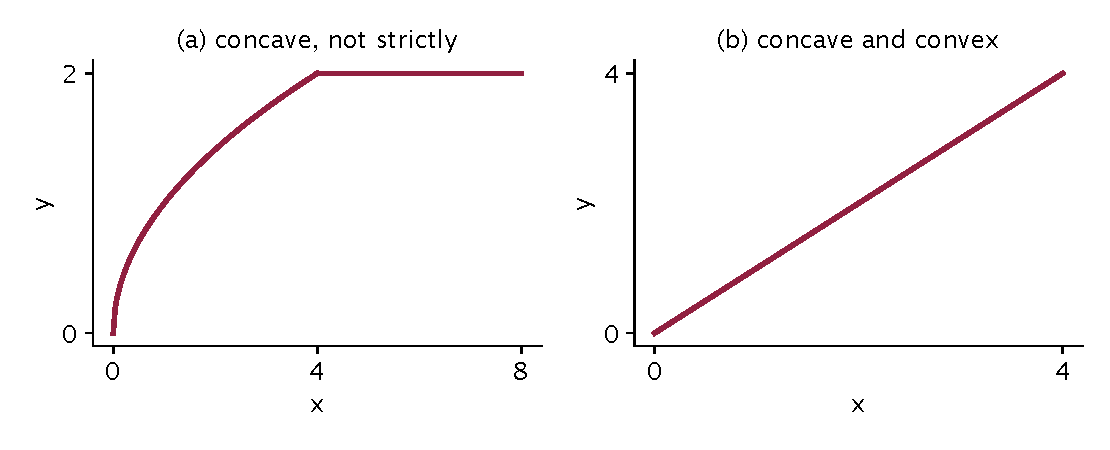
\includegraphics[width=0.8\textwidth,alt={Two panels. Panel a: a curve that rises like a square root and then continues as a flat horizontal line, so it is concave but contains a straight segment. Panel b: a straight line through the origin with slope 1, which is both concave and convex}]{../../latex/fig/concave-examples.pdf}
\end{center}

% Question 4
\item[4.] $y = a - \dfrac{b}{c + x}$
\begin{enumerate}
\item[(a)] $\dfrac{dy}{dx} = \dfrac{b}{(c + x)^{2}} > 0$ and $\dfrac{d^{2}y}{dx^{2}} = -\dfrac{2b}{(c + x)^{3}} < 0$, so the function is increasing and strictly concave.
\item[(b)] At $x = 0$, $y = a - b/c$.
\item[(c)] As $x \to \infty$, $b/(c + x) \to 0$, so $y \to a$. The graph rises from $a - b/c$ toward the horizontal asymptote $y = a$, flattening as it goes.
\end{enumerate}
As a consumption function with income $x$: consumption should be positive at zero income, which requires $ac > b$, and the marginal propensity to consume $dy/dx$ should be less than $1$ at every income level, which requires $b/c^{2} < 1$, that is, $b < c^{2}$.

% Question 5
\item[5.] $f(x)$ must be a constant, say $f(x) = 1$; every point is a stationary point. $g(x)$ could be $g(x) = x^{2} - 6x + 10$, which has a single stationary point at $x = 3$. The difference: $f$ is stationary everywhere, whereas $g$ is stationary only at $x = 3$.
\begin{center}
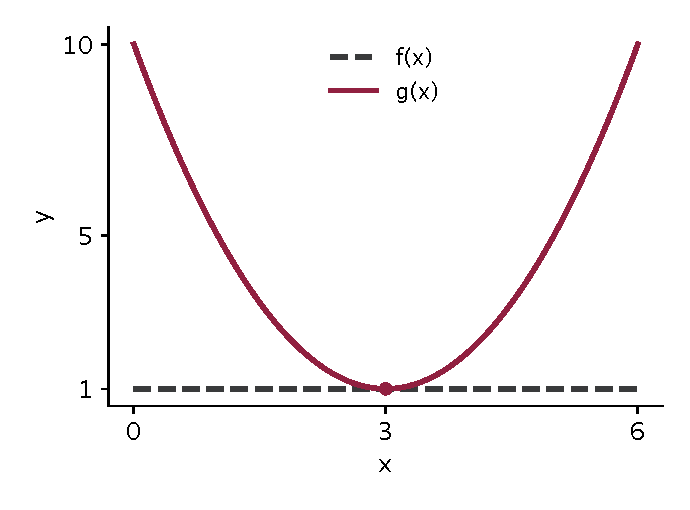
\includegraphics[width=0.45\textwidth,alt={A dashed horizontal line f of x equals 1 and a maroon parabola g of x with its minimum at (3, 1), marked by a dot, touching the line there}]{../../latex/fig/stationary-points.pdf}
\end{center}

\end{enumerate}

\underline{Exercise 9.4}
\begin{enumerate}
% Question 1
\item[1.]
\begin{enumerate}
\item[(b)] $y = x^{3} + 6x^{2} + 9$
\[y' = 3x^{2} + 12x = 3x(x + 4) = 0 \;\Rightarrow\; x^{*} = 0, -4; \qquad y'' = 6x + 12\]
$y''(0) = 12 > 0$, so $y(0) = 9$ is a relative minimum. $y''(-4) = -12 < 0$, so $y(-4) = 41$ is a relative maximum.
\item[(d)] $y = \dfrac{2x}{1 - 2x}$. By the quotient rule,
\[y' = \frac{2(1 - 2x) - 2x(-2)}{(1 - 2x)^{2}} = \frac{2}{(1 - 2x)^{2}}\]
which is never zero. There is no stationary point, so there are no relative extrema. The function is increasing on each side of $x = 1/2$.
\end{enumerate}

% Question 2
\item[2.] Let $L$ be the side parallel to the wall and $W$ the two sides perpendicular to it. The netting constraint is $L + 2W = 64$, so $L = 64 - 2W$ and the area is
\[A = LW = (64 - 2W)W = 64W - 2W^{2}\]
\[\frac{dA}{dW} = 64 - 4W = 0 \;\Rightarrow\; W^{*} = 16, \quad L^{*} = 32\]
Since $d^{2}A/dW^{2} = -4 < 0$, this is a maximum (the area function is strictly concave, so it is the global maximum). The largest area is $32 \times 16 = 512$ square feet.

% Question 3
\item[3.]
\begin{enumerate}
\item[(a)] Yes: $a = 1/3 > 0$, $b = -7 < 0$, $c = 111 > 0$, $d = 50 > 0$, and $b^{2} = 49 < 3ac = 111$.
\item[(b)] From the demand function, $P = 100 - Q$, so $R = PQ = (100 - Q)Q = 100Q - Q^{2}$.
\item[(c)] $\pi = R - C = 100Q - Q^{2} - \tfrac{1}{3}Q^{3} + 7Q^{2} - 111Q - 50 = -\tfrac{1}{3}Q^{3} + 6Q^{2} - 11Q - 50$
\item[(d)]
\[\frac{d\pi}{dQ} = -Q^{2} + 12Q - 11 = 0 \;\Rightarrow\; (Q - 1)(Q - 11) = 0 \;\Rightarrow\; Q = 1 \text{ or } 11\]
$\dfrac{d^{2}\pi}{dQ^{2}} = -2Q + 12$ is $10 > 0$ at $Q = 1$ (a minimum) and $-10 < 0$ at $Q = 11$ (a maximum). So $Q^{*} = 11$.
\item[(e)] $\pi(11) = -\tfrac{1}{3}(1331) + 6(121) - 11(11) - 50 = 334/3 \approx 111.33$.
\end{enumerate}

% Question 5
\item[5.] $\pi(Q) = hQ^{2} + jQ + k$
\begin{enumerate}
\item[(a)] $\pi(0) = k$, so $k < 0$.
\item[(b)] $\pi'(Q) = 2hQ + j$ and $\pi''(Q) = 2h$, so strict concavity requires $h < 0$.
\item[(c)] The critical point is $Q^{*} = -j/(2h)$. With $h < 0$, we need $j > 0$ to make $Q^{*} > 0$.
\end{enumerate}

\end{enumerate}
